\subsection{Modelo de Android}
\begin{frame}
 \begin{center}
  \LARGE Modelo de Android
 \end{center}
\end{frame}
\begin{frame}
 \frametitle{Modelo de Android}
 \begin{itemize}
  \item Android es un sistema operativo de código abierto, diseñado para dispositivos móviles y desarrollado por Google junto con la Open Handset Alliance.\pause
  \item Su arquitectura sigue el estilo arquitectónico conocido como Sistemas Estratificados: los distintos componentes se agrupan en capas según su nivel de abstracción, conformando una jerarquía. \pause Las capas inferiores contienen componentes ligados al \textit{hardware}, mientras que las capas superiores agrupan componentes ligados con tareas de más alto nivel.\pause
  \item Cada aplicación se ejecuta en un \emph{entorno aislado}\footnote{Traducción propuesta para el término \textit{sandbox}.}, forzando a que solo pueda tener acceso irrestricto a sus propios recursos.
 \end{itemize}
 \begin{itemize}
  \item Los recursos que provee Android sólo pueden ser accedidos mediante una SS-API\footnote{\textit{Security Sensitive API}, por sus siglas en inglés.} con un doble objetivo: \pause tenerlos aislados y permitir cierta granularidad de seguridad sobre ellos.\pause
  \item El mecanismo para el acceso a estas SS-API se llama Permisos.
 \end{itemize}
\end{frame}
\begin{frame}
 \frametitle{Modelo de Android}
 \begin{itemize}
  \item Podemos clasificar los permisos según el riesgo implícito al otorgarlos, resultando las siguientes cuatro categorías: \emph{Normal}, \emph{Dangerous}, \emph{Signature} y \emph{Signature/System}. \pause El presente informe se centra en los permisos \emph{Normales} y \emph{Peligrosos}; cómo se otorgan y cómo se deniegan.\pause
  \item En las versiones anteriores a Android Marshmallow, al prepararse para instalar una aplicación, el sistema operativo mostraba un diálogo al usuario indicando los permisos solicitados y se le consultaba si deseaba continuar con la instalación.\pause
  \item En caso afirmativo, el sistema otorgaba todos los permisos solicitados e instalaba la aplicación. \pause En el caso contrario, no se instalaba la aplicación.\pause
  \item El usuario quedaba preso si quería instalar una aplicación: no podía otorgar o denegar permisos individuales; debía otorgar o denegar todos los permisos solicitados como un bloque. \pause Una vez concedidos, los permisos seguían vigentes mientras la aplicación estuviera instalada. Solo se eliminaban si se desinstala dicha aplicación.
 \end{itemize}
\end{frame}
\begin{frame}
 \frametitle{Modelo de Android}
 \begin{itemize}
  \item A partir de la versión 6.0 se propone un nuevo modelo de permisos, donde los usuarios pueden administrar en tiempo de ejecución los permisos \emph{peligrosos} requeridos por una aplicación. \pause En este modelo, los permisos se agrupan para facilitar el control de la privacidad de los usuarios.\pause
 \end{itemize}
 \begin{figure}[btp]
    \centering
    \begin{subfigure}{0.2\linewidth}
        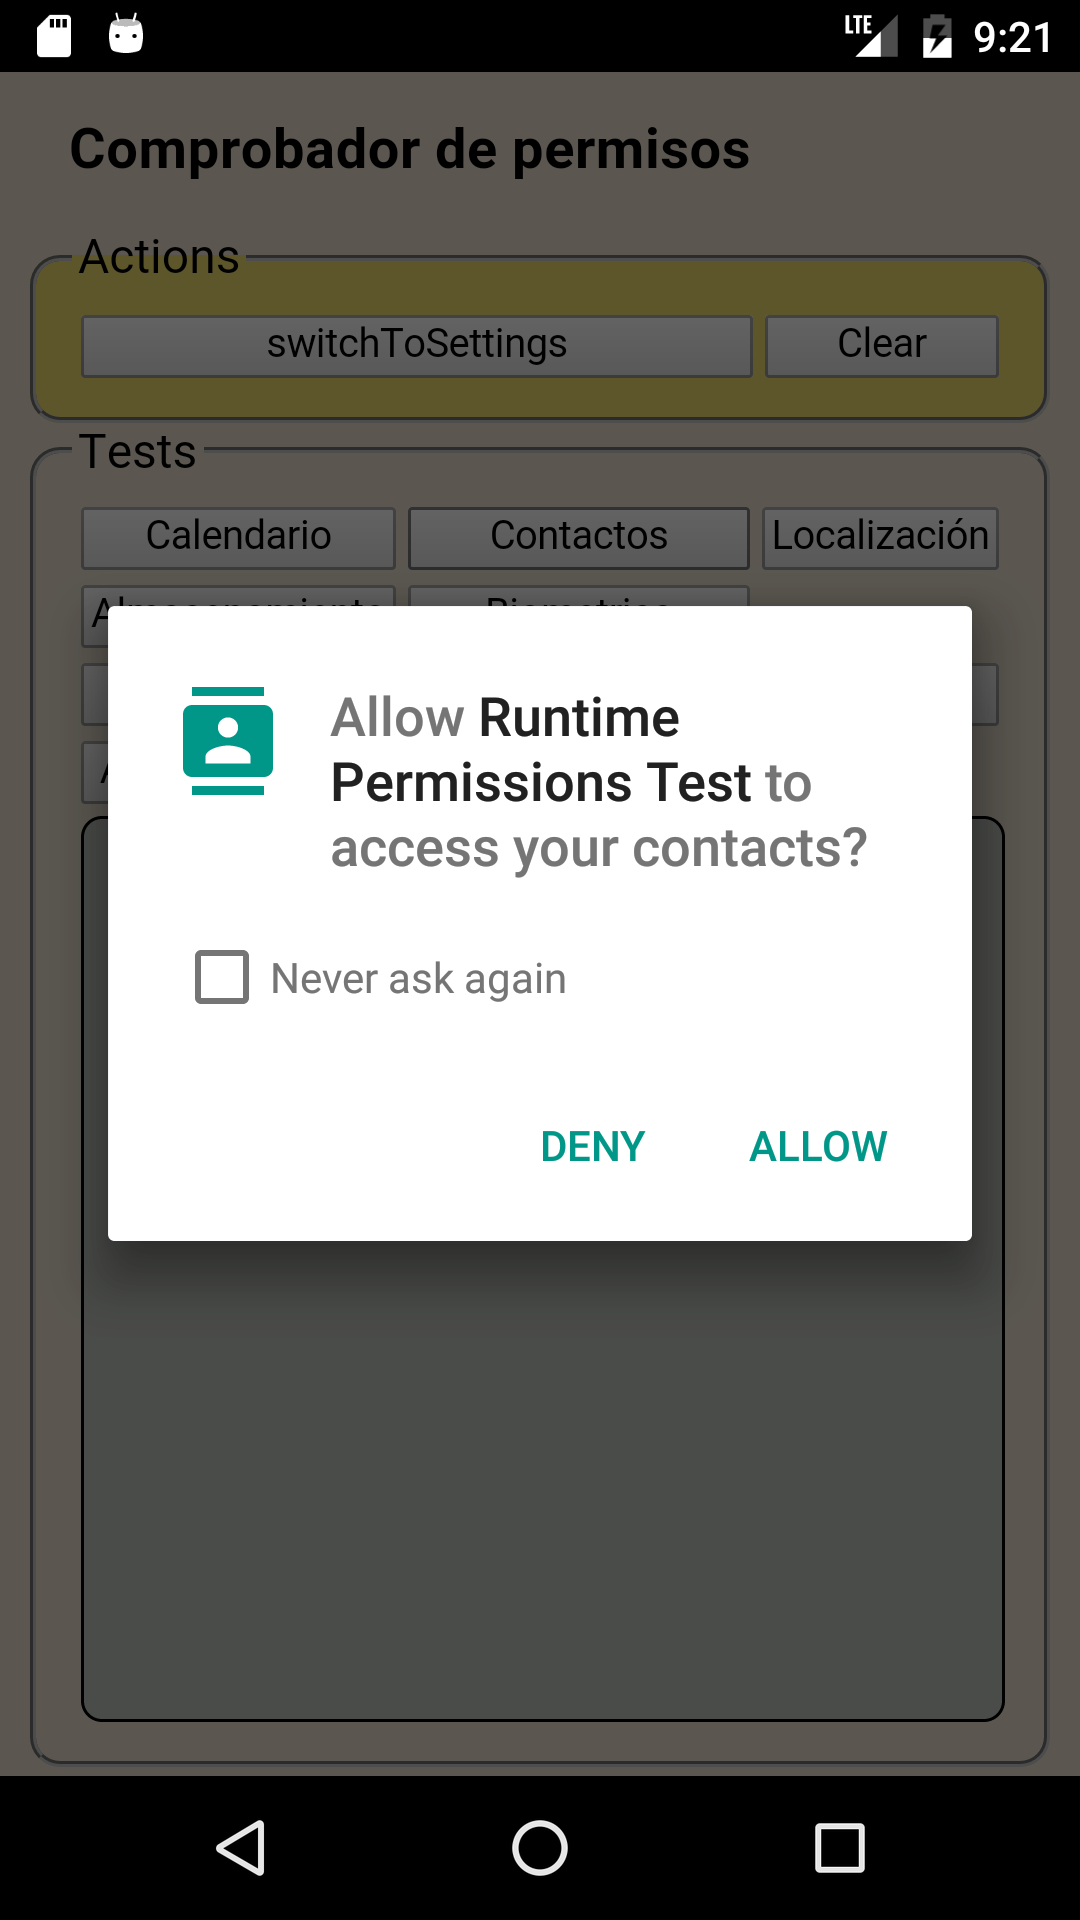
\includegraphics[width=\linewidth]{allow_contact}
        \caption{Solicitud de un permiso.}
    \end{subfigure}
    \begin{subfigure}{0.2\linewidth}
        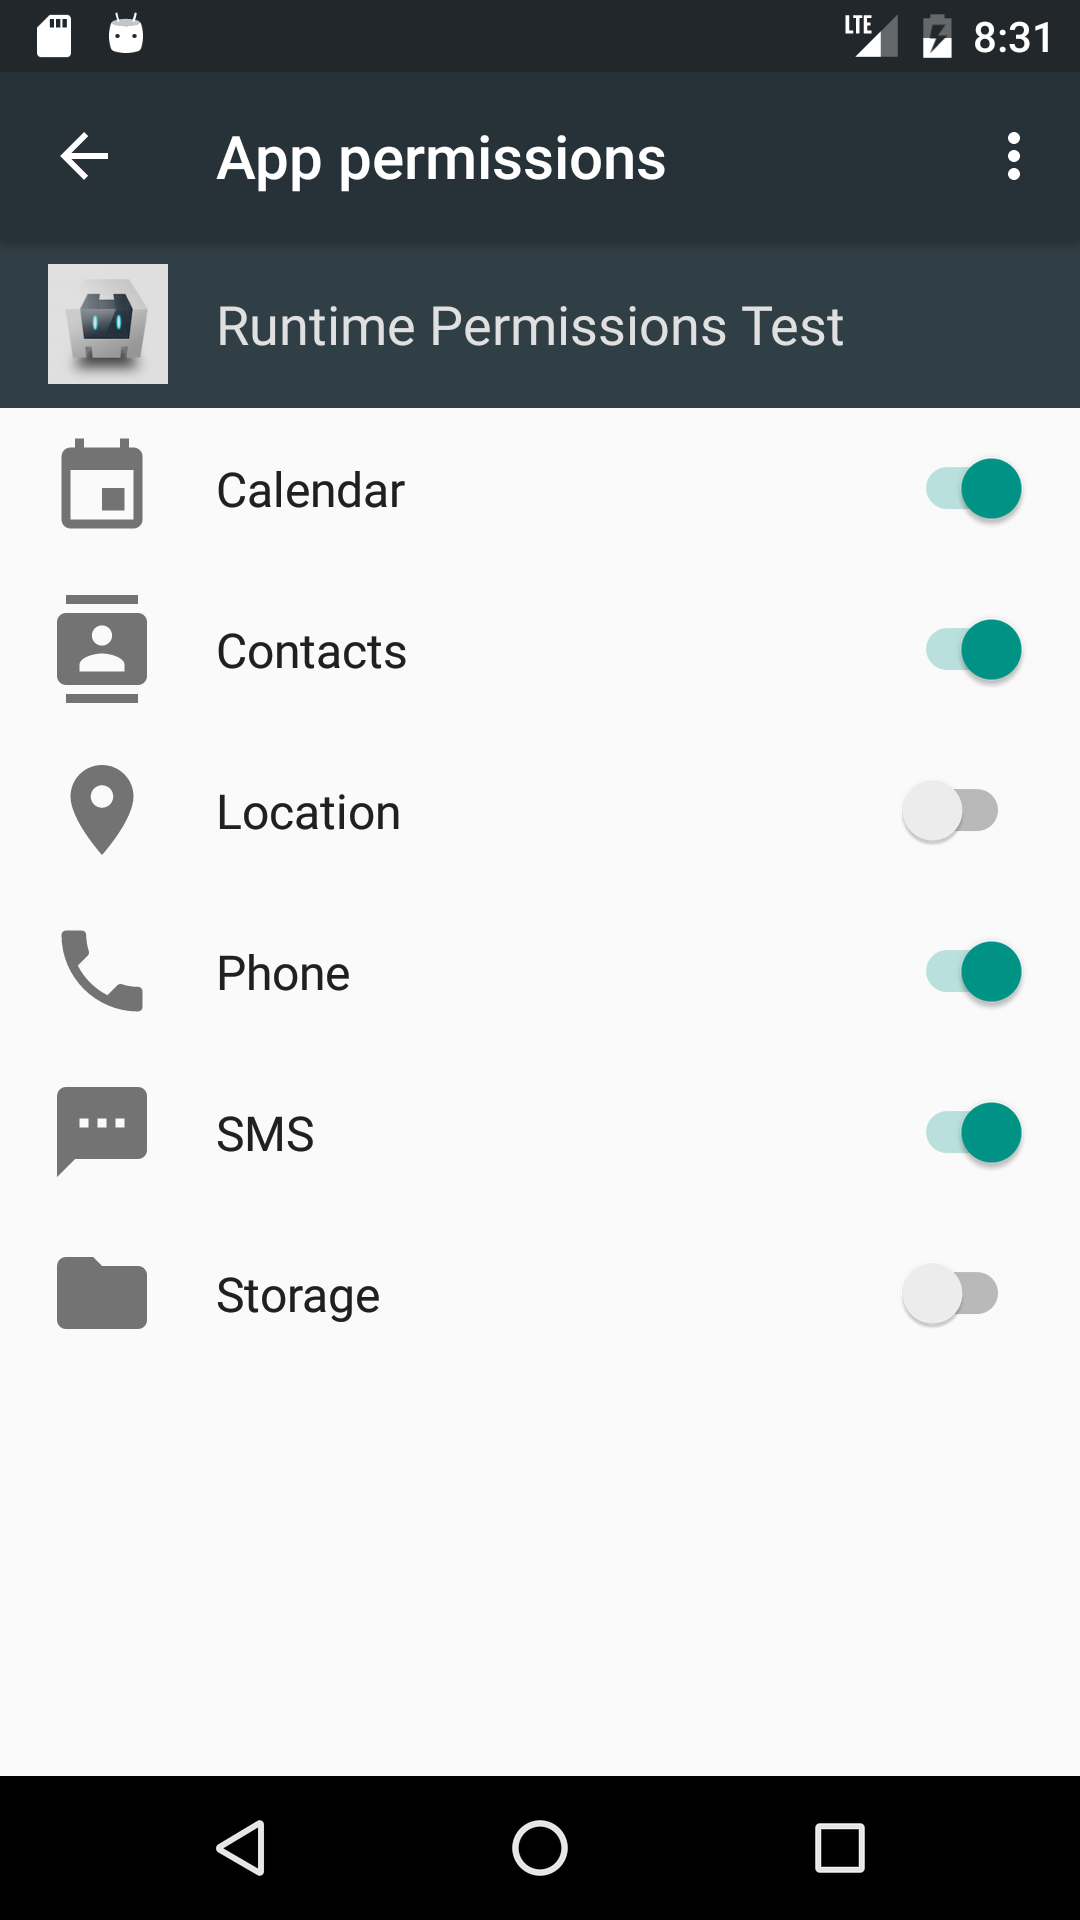
\includegraphics[width=\linewidth]{app-permissions}
        \caption{Listado de los permisos.}
	\end{subfigure}
	\begin{subfigure}{.5\linewidth}
	 \begin{small}\pause
	 \begin{itemize}
	  \item A partir de esta versión, durante la instalación de una aplicación se le otorgan todos los permisos \emph{normales} y ningún permiso \emph{peligroso}.\pause
  \item Como consecuencia de esto, cada vez que una aplicación necesita acceder a un recurso protegido por un permiso \emph{peligroso}, tiene que solicitarlo en tiempo de ejecución.
    \end{itemize}
    \end{small}
   \end{subfigure}
 \end{figure}
\end{frame}